\documentclass[a4paper,oneside]{scrarticle}

\usepackage[left=3cm,right=3cm,top=2cm,bottom=2.25cm]{geometry}
\usepackage[ngerman]{babel}
\usepackage{amsmath}
\usepackage{amsfonts}
\usepackage{amssymb}
\usepackage{mathtools}
\usepackage{graphicx}
%\graphicspath{ {./images/} }
\addto\captionsngerman{\renewcommand{\figurename}{Fig.}}


\begin{document}
	\begin{flushleft}
		Bach Nguyen, Johannes Roloff - HTWK Leipzig - INB
	\end{flushleft}
	\begin{center}
		\begin{LARGE}
			\textbf{Station 5 Evaluation}
		\end{LARGE}
	\end{center}
	\section*{Einordnung der Aufgabe im Prozess}
	\begin{figure} [h]
		\centering
		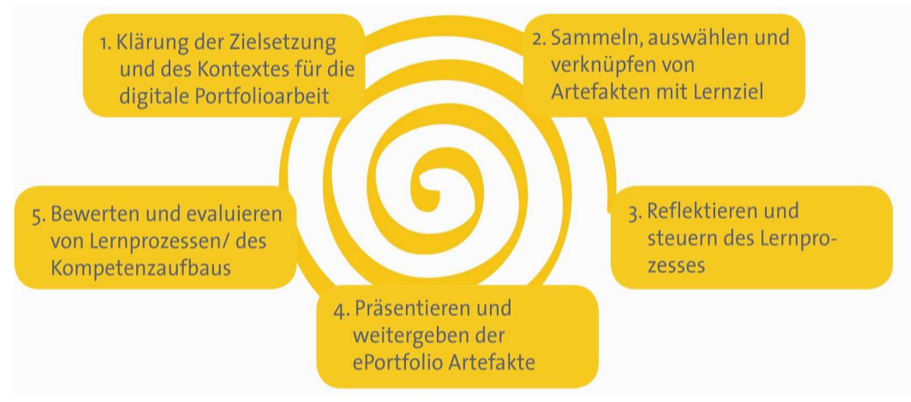
\includegraphics[width=0.7\linewidth]{e-portfolio-prozesse-schaffert}
		\caption{Prozesse der Portfolio-Arbeit (Schaffert et al. 2007, S. 79)}
		\label{fig:e-portfolio-prozesse-schaffert}
	\end{figure}
	\begin{figure}[h]
		\centering
		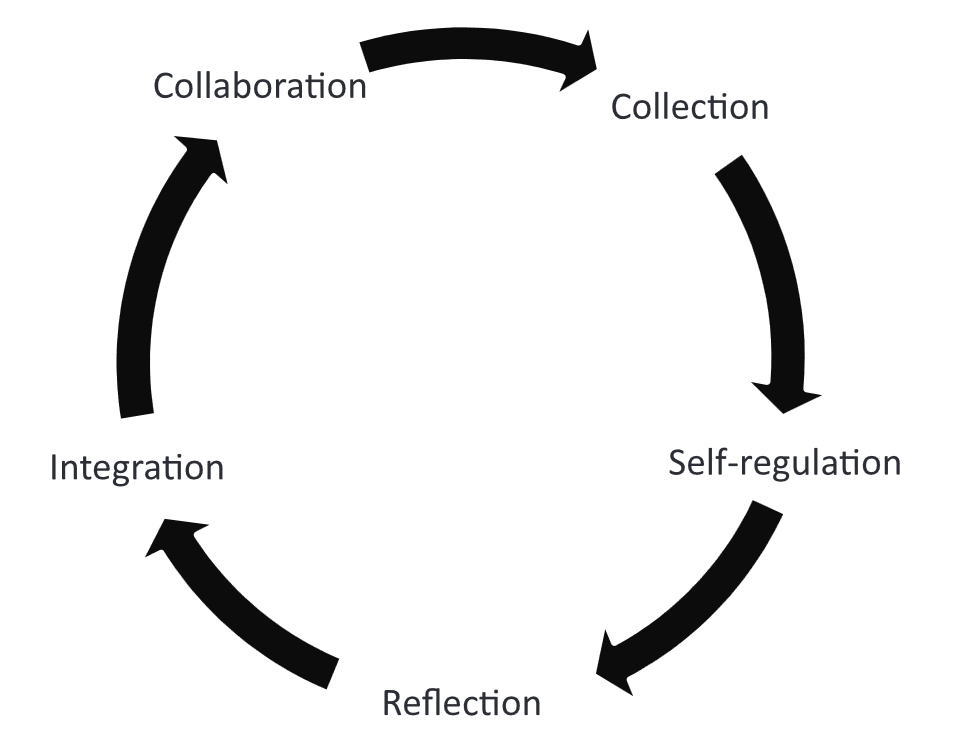
\includegraphics[width=0.5\linewidth]{cycle-of-documented-lifelong-learning-Jensen}
		\caption{cycle of documented lifelong learning (Jensen,Treuer 2014)}
		\label{fig:cycle-of-documented-lifelong-learning-jensen}
	\end{figure}
	\begin{figure}[h]
		\centering
		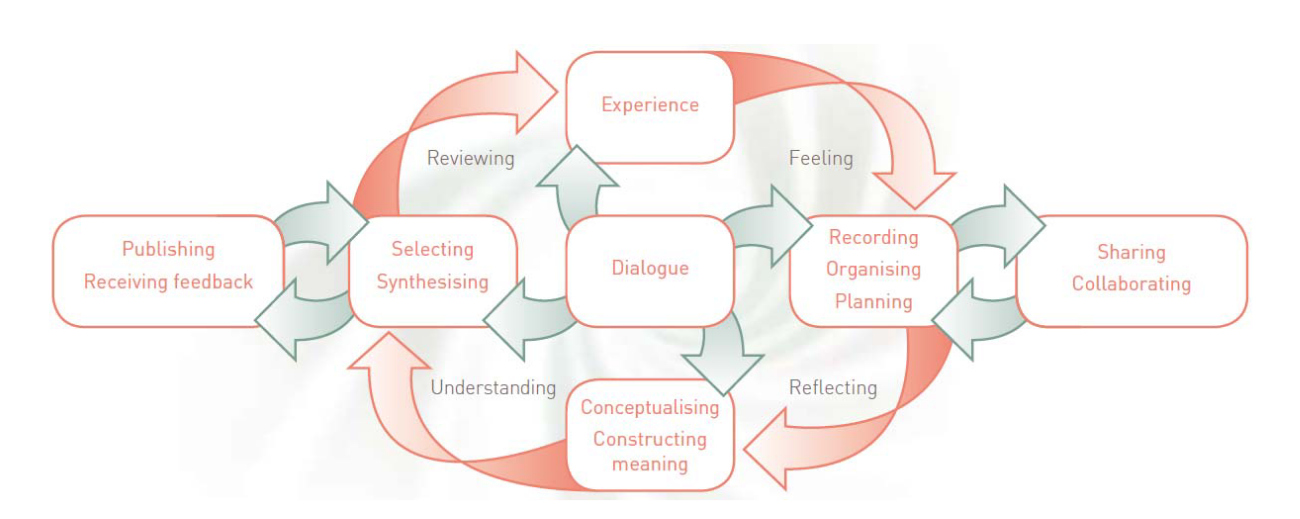
\includegraphics[width=0.8\linewidth]{model-of-e-portfolio-based-learning}
		\caption{A model of e-portfolio-based learning (JISC 2008, S. 9)}
		\label{fig:model-of-e-portfolio-based-learning}
	\end{figure}

	\pagebreak 
	
	\section*{Einleitung}
	An dieser Stelle beginnt die Evaluationsphase. Bewerte Deinen eigenen Lernfortschritt. Dies ist eine weiterführende Art der Reflexion. 
	
	\section*{Aufgabenstellung}

	\begin{enumerate}
		\item Schaue zuerst zurück auf das ausgewählte Modul. Schreibe einen Evaluationsbericht über deinen Lernfortschritt. Nutze dazu Modulux und beantworte, ob du die Lernziele erreicht hast. Beantworte ebenfalls folgende Fragen.
		\begin{enumerate}
			\item Spiegelt sich mein Gelerntes in meiner Note wieder?
			\item Habe ich meine Lernziele erreicht?
			\item Was waren fördernde und hemmende Faktoren gewesen?
			\item Habe ich die Lernziele im Modulhandbuch erreicht?
			\item In welcher Form könnte mein angeeignetes Wissen, weiterhin in meinem Leben nützlich sein?
		\end{enumerate}
		\item Für dein Studium bis zu diesem Zeitpunkt, schreibe einen Evaluationsbericht. Beantworte dabei folgende Fragen.
		\begin{enumerate}
			\item Spiegelt sich mein Gelerntes in meiner Note wieder?
			\item Habe ich meine Lernziele erreicht?
			\item Was waren fördernde und hemmende Faktoren gewesen?
			\item Habe ich die Lernziele im Modulhandbuch erreicht?
			\item In welcher Form könnte mein angeeignetes Wissen, weiterhin in meinem Leben nützlich sein?
		\end{enumerate}

	\end{enumerate}


\end{document}
